\chapter{Aspartate's role in cellular metabolism of the proliferating cell}
\label{chap1}
\textit{Metabolism, the sum of chemical reactions occurring inside living organisms.}
%\textit{Metabolism, the sum of the chemical reactions occurring inside a cell} (abridged version of the definition by Hans Kornberg \cite{BriMetabDef}).

\section{Introduction}
Most of metabolism is \textit{cellular metabolism}, occurring within the confines of a cell, to bring together metabolites and enzymes at a sufficient concentration to enable production of energy and large biomolecules such as proteins, DNA/RNA and lipids.
It follows, that \textit{cancer metabolism} is metabolism occurring inside cancer cells.
However, most often the term is used comparatively to highlight the differences between metabolism in healthy and cancerous cells, with the assumption that such differences can be targeted therapeutically to provide anti-cancer treatments \cite{Vander_Heiden2011-ce, Hamanaka2012-kw, Luengo2017-kf, Vasan2020-yr}.
Cancer metabolism is most often associated with the ``Warburg effect'', an observation made during the 1920s by Otto Warburg that cancer cells in the presence of ample oxygen ferment glucose to lactate and therefore also known as ``aerobic glycolysis'' \cite{warburg1926stoffwechsel, Chandel2021-rf}.
Since then, many researchers have rediscovered this phenomenon and attempted to explain this squandering of glucose in many ways.
At present it suffices to say that aerobic glycolysis in cancer cells is not due to mitochondria dysfunction and that other non-cancerous rapidly proliferation cells like T and embryonic stem cells also engage in abundant lactate production.

In the context of this thesis the Warburg effect serves as an illustration that little, if any, difference can be observed between metabolism of the cancer cell and an appropriately matched proliferating cell.
This is the Achilles' heel of the therapeutic ambitions of cancer metabolism, but it also suggests that many lessons about basic cellular metabolism can be learned by studying cancer cells.
Indeed, this is becoming increasingly popular because of the large palette of well characterized cancer cell lines that are rapidly dividing, easy to passage and commercially available.
Thus, making gene knockouts, protein over-expression, inhibitor treatments, CRISPR screens etc. available with relative ease.
In this thesis, cancer cell lines are also used in such way, with the objective of more broadly generalizing about cellular metabolism of proliferating cells.



\section{The metabolic rational for aerobic glycolysis}
Many reasons have been provided to rationalize the apparent energetic waste of aerobic glycolysis \cite{Vander_Heiden2009-uf, OBrien2013-dt, Huberts2012-gk, Zhuang2011-nm, Pfeiffer2001-pu}.
Interesting parallels have been drawn between proliferating cells of unicellular and multicellular origin as a way of rationalizing aerobic glycolysis \cite{Vander_Heiden2009-uf}.
In the context of yeast, aerobic glycolysis is also known as the Crabtree effect; a feature displayed by some strains but not by others \cite{De_Deken1966-bp}.
The effect is also found in bacteria where acetate is secreted in what is known as the acetate switch \cite{Wolfe2005-cy}.
A hypothetical explanation of the Crabtree effect in unicellular organisms was proposed by modeling the protein synthesis cost and pathway efficiency to derive an estimate of ATP produced per unit time per unit protein required \cite{Molenaar2009-go}.
In this ``proteome allocation'' hypothesis, the cost of ATP production through aerobic glycolysis is lower than oxidative phosphorylation because glycolytic enzymes are few and fast whereas oxidative phosphorylation requires many more enzymes with slower conversion rates.
Although ATP production per glucose through aerobic glycolysis is 2 vs. approximately 36 for oxidative phosphorylation, the cost of enabling oxidative phosphorylation in human cells is enormous with around 50 proteins required for complex I structure and assembly \cite{Sharma2009-ws}, 11 subunits in complex III \cite{Iwata1998-td}, 14 subunits in complex IV \cite{Signes2018-df}, 29 proteins in ATPase \cite{He2018-rl} and a long list of regulatory proteins.
Indeed, it was later experimentally determined that aerobic glycolysis was approximately twice as efficient as oxidative phosphorylation when comparing the protein demands in \textit{E.coli} \cite{Basan2015-bq}.
However, this simple conclusion is likely more complicated since some Crabtree positive and negative yeast strains have a similar growth rates; an observation that has been explained by different translation efficiencies caused by usage of different ribosomal subunit variants \cite{Malina2021-lb}.

The parallels between aerobic glycolysis in unicellular and multicellular organisms are many but so are the differences.
Multicellular organisms have evolved towards a high degree of regulation at the expense of efficiency and their metabolism is often compartmentalized such that some tissues handle the waste of others e.g. the Cori cycle of lactate and the urea cycle of ammonia.
Human cells also experience a constant supply of amino acids from the blood and thus do not incur the same cost of protein synthesis as a yeast cell growing with ammonium as the sole source of nitrogen.
Therefore, it is unclear if the proteome allocation hypothesis even applies to cancer cells.

Rather than being ATP limited, cancer cells appear to be oversupplied with ATP \cite{Scholnick1973-wx}.
High ATP shifts the balance between ATP and AMP which inhibits the glycolytic enzyme phosphofructokinase (PFK) \cite{Dunaway1983-ee}.
Conversely, limiting ATP synthesis from ATPase using oligomycin leads to lower ATP/ADP, resulting in enhanced forward driving force of glycolysis \cite{Park2019-cg}.
Tumor up-regulated genes leading to increased ATP consumption through ER UDPase relieves the cell of high ATP and increase both glycolysis and proliferation \cite{Fang2010-mj, Israelsen2010-ke}.
It has also been shown that when pyruvate oxidation is pharmacologically induced in cancer cells it leads to lower \NAD/NADH levels, increased mitochondrial membrane potential and lower proliferation that can all be reversed by uncoupling the mitochondrial membrane potential using an ionophore \cite{Luengo2021-kb}.
The proposed mechanism is that the ATP/ADP (or ATP/AMP) ratio is high at baseline and that more mitochondrial NADH and proton pumping leads to higher membrane potential because ATPase is substrate limited due to low ADP supply.
That proliferation can be rescued by relieving the mitochondrial membrane potential directly through uncoupling or increasing the ATP consumption through increased ATP hydrolysis by Na\textsuperscript{+}/K\textsuperscript{+}-ATPase demonstrates that ATP is not limiting for cancer cell proliferation.

Consensus among contemporary research appear to be that cancer cells maintain high flux through glycolysis to drive the pentose-phosphate pathway, serine synthesis and generation of NADPH, and as a side-product an abundance of lactate is produced to regenerate the \NAD{} cofactor consumed by glycolysis \cite{Vander_Heiden2017-eq, Chandel2021-rf}.




\section{Environmental limitations to cancer cell proliferation}
The cellular metabolism of proliferating cells must be calibrated to provide components for cell copying.
Ordered by biomass abundance, these components are amino acids, nucleotides and fatty acids followed by the plethora of lower abundance molecules that make up a cell.
In culture, protein and lipid biomass is mostly scavenged by uptake of amino acids and lipids from the media, whereas nucleotides are primarily derived from glucose metabolism \cite{Hosios2016-us}.

For the NCI-60 set of cancer cell lines, proliferation data exists both for cells in culture and cells transplanted into immunodeficient mice (figure \ref{fig:ch1:prlfr_contr}).
For the cells in culture, they tend to double once a day, while when xenografted it takes approximately five times as long.
Some of which have grown in culture for decades, so it is not surprising that they prefer the cell culture environment over being under the skin of a mouse.
Could some of this difference be explained by metabolic differences?
One piece of evidence in support of this is that cancer cell lines engineered with the ability to scavenge aspartate from the environment outgrow their non-aspartate scavenging counterparts when grown as tumors in mice but not in culture \cite{Sullivan2018-gz, Garcia-Bermudez2018-mj}.
This would suggest that aspartate availability is limiting tumor growth, thus explaining some of the difference observed in figure \ref{fig:ch1:prlfr_contr}.

\begin{figure}
    \centering
    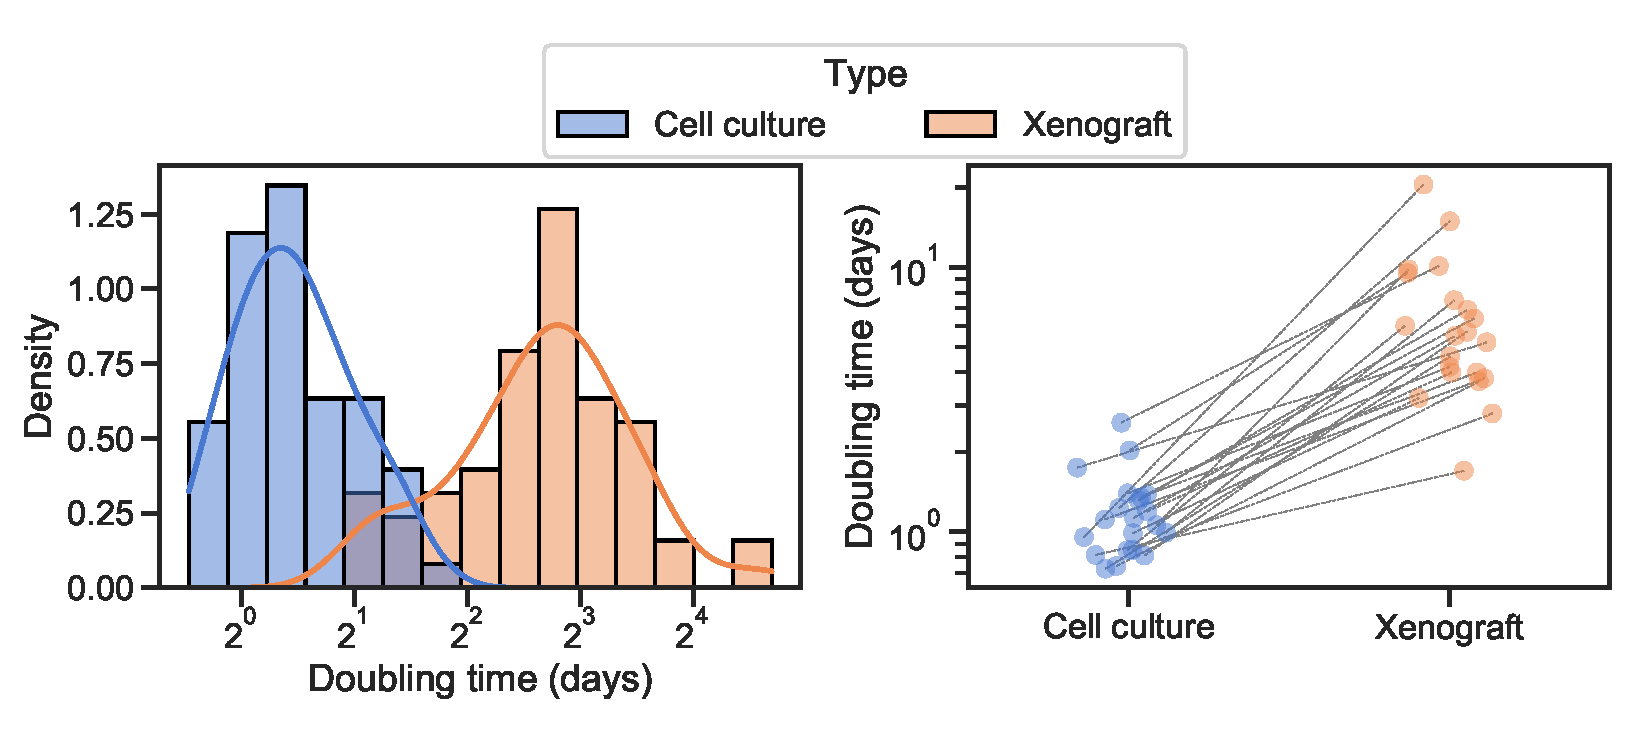
\includegraphics[width=0.70\textwidth]{figures/chap1/prlfr_contr.pdf}
    \caption[NCI-60 cancer cell line doubling time in cell culture vs. xenografts.]{
    NCI-60 cancer cell line doubling time in cell culture vs. xenografts.
    Left plot: distribution of doubling time of all NCI-60 cells in culture vs. those with data in xenografts.
    Right plot: paired doubling times for those cell lines with data in xenografts.
    Paired data connected by dashed lines.
    Cell culture data from NCI \cite{NCI60}, xenograft data from Charles River \cite{CR_tumor}.
    }
    \label{fig:ch1:prlfr_contr}
\end{figure}




\section{Cellular metabolism requires redox balance}
A well-known metabolic difference between cells in culture and in a tumor is the oxygen tension.
Cells in culture experience oxygen levels close to atmospheric air whereas cells in tissues experience 2-10 fold lower oxygen \cite{Ast2019-hh}.
Due to poor vascularization, cells in a tumor experience another 2-10 fold lower oxygen than their host tissue \cite{McKeown2014-tt}.
For mammalian cells oxygen is the principal electron acceptor and thus this profound decrease in oxygen tension could lead to decreased respiration.
Lower respiration results in lower ATP production from oxidative phosphorylation and lower capacity to regenerate \NAD.
As noted previously, ATP production does not appear to limit proliferation; however, redox imbalance could. 

Cellular redox is governed by the co-factors \NADP{} and \NAD{} and their redox status defined by the ratio of oxidized to reduced: NAD(P)\textsuperscript{+}/NAD(P)H.
The two redox pools are separate due to the absence of transhydrogenase activity and tight regulation around metabolic reactions ending in conversion.
Generally speaking, \NAD{} is consumed in catabolic reactions such as glycolysis and TCA cycling and NADPH is consumed in anabolic reactions such as amino acid, fatty acid and nucleotide synthesis.
NADPH is primarily generated through the pentose-phosphate pathway \cite{Chen2019-ex, Ghergurovich2020-sh, Zhang2021-mg}.
\NAD{} is generated in several reactions in the TCA cycle and glycolysis and regenerated through respiration.
For yeast, biosynthesis of 100 g cells from glucose and ammonia has been estimated to leads to a net production of NADH and a net consumption of NADPH described by the following stoichiometry \cite{Bruinenberg1983-tn, Van_Dijken1986-zp}:
\begin{center}
737 C\textsubscript{6}H\textsubscript{12}O\textsubscript{6} + 680 NH\textsubscript{3} + 6 H\textsubscript{2}SO\textsubscript{4} + 931 NADPH + 1349 \NAD{} \Rightarrow \newline
1000 C\textsubscript{4}H\textsubscript{7.32}O\textsubscript{2.24}N\textsubscript{0.68}S\textsubscript{0.006} (100 g cells) + 424 CO\textsubscript{2} + \newline931 \NADP{} + 1349 NADH + 1358 H\textsubscript{2}O + 418 H\textsuperscript{+}
\end{center}

However, besides glucose, mammalian cells have access to fatty acids and amino acids from the blood supply and therefore most of the NADPH consumption for anabolic processes can be avoided.
Nucleosides and nucleobases on the other hand are not abundant in serum \cite{Traut1994-vu} (appendix \ref{fig:app_ch1:pig_nucl_conc}) and thus need to be synthesized.
Most amino acids are available in serum and can be taken up to fulfill the protein synthesis demand of cancer cells; however, aspartate is an exception due to low cell permeability and low serum concentrations.
Glutamate has similar low cell permeability but is readily generated through deamination by the enzyme glutaminase.
Aspartate is neither cell permeable nor generated through asparagine deamination in most cell lines \cite{Sullivan2018-gz} and thus has to be synthesized from either glucose or glutamine with a net consumption of \NAD{} (figure \ref{fig:ch1:redox_biomass}).

Under standard cell culture conditions, respiration is sufficient to regenerate \NAD{} to allow unconstrained aspartate synthesis; however, the mitochondrial electron transport chain can be inhibited with various drugs (figure \ref{fig:ch1:redox_biomass}) to constrain aspartate production and limit proliferation.
The redox imbalance created by inhibited respiration can conveniently be rescued by providing an exogenous electron acceptor such as pyruvate or alpha-ketobutyrate and these tools have been frequently used to study redox imbalance and its effect on aspartate synthesis \cite{Birsoy2014-em, Sullivan2015-xf, Birsoy2015-pg, Gui2016-ca, Garcia-Bermudez2018-mj, Alkan2018-zv, Diehl2019-um, Yang2020-fs, Luengo2021-kb, Garcia-Bermudez2022-qn}.

\begin{figure}
    \centering
    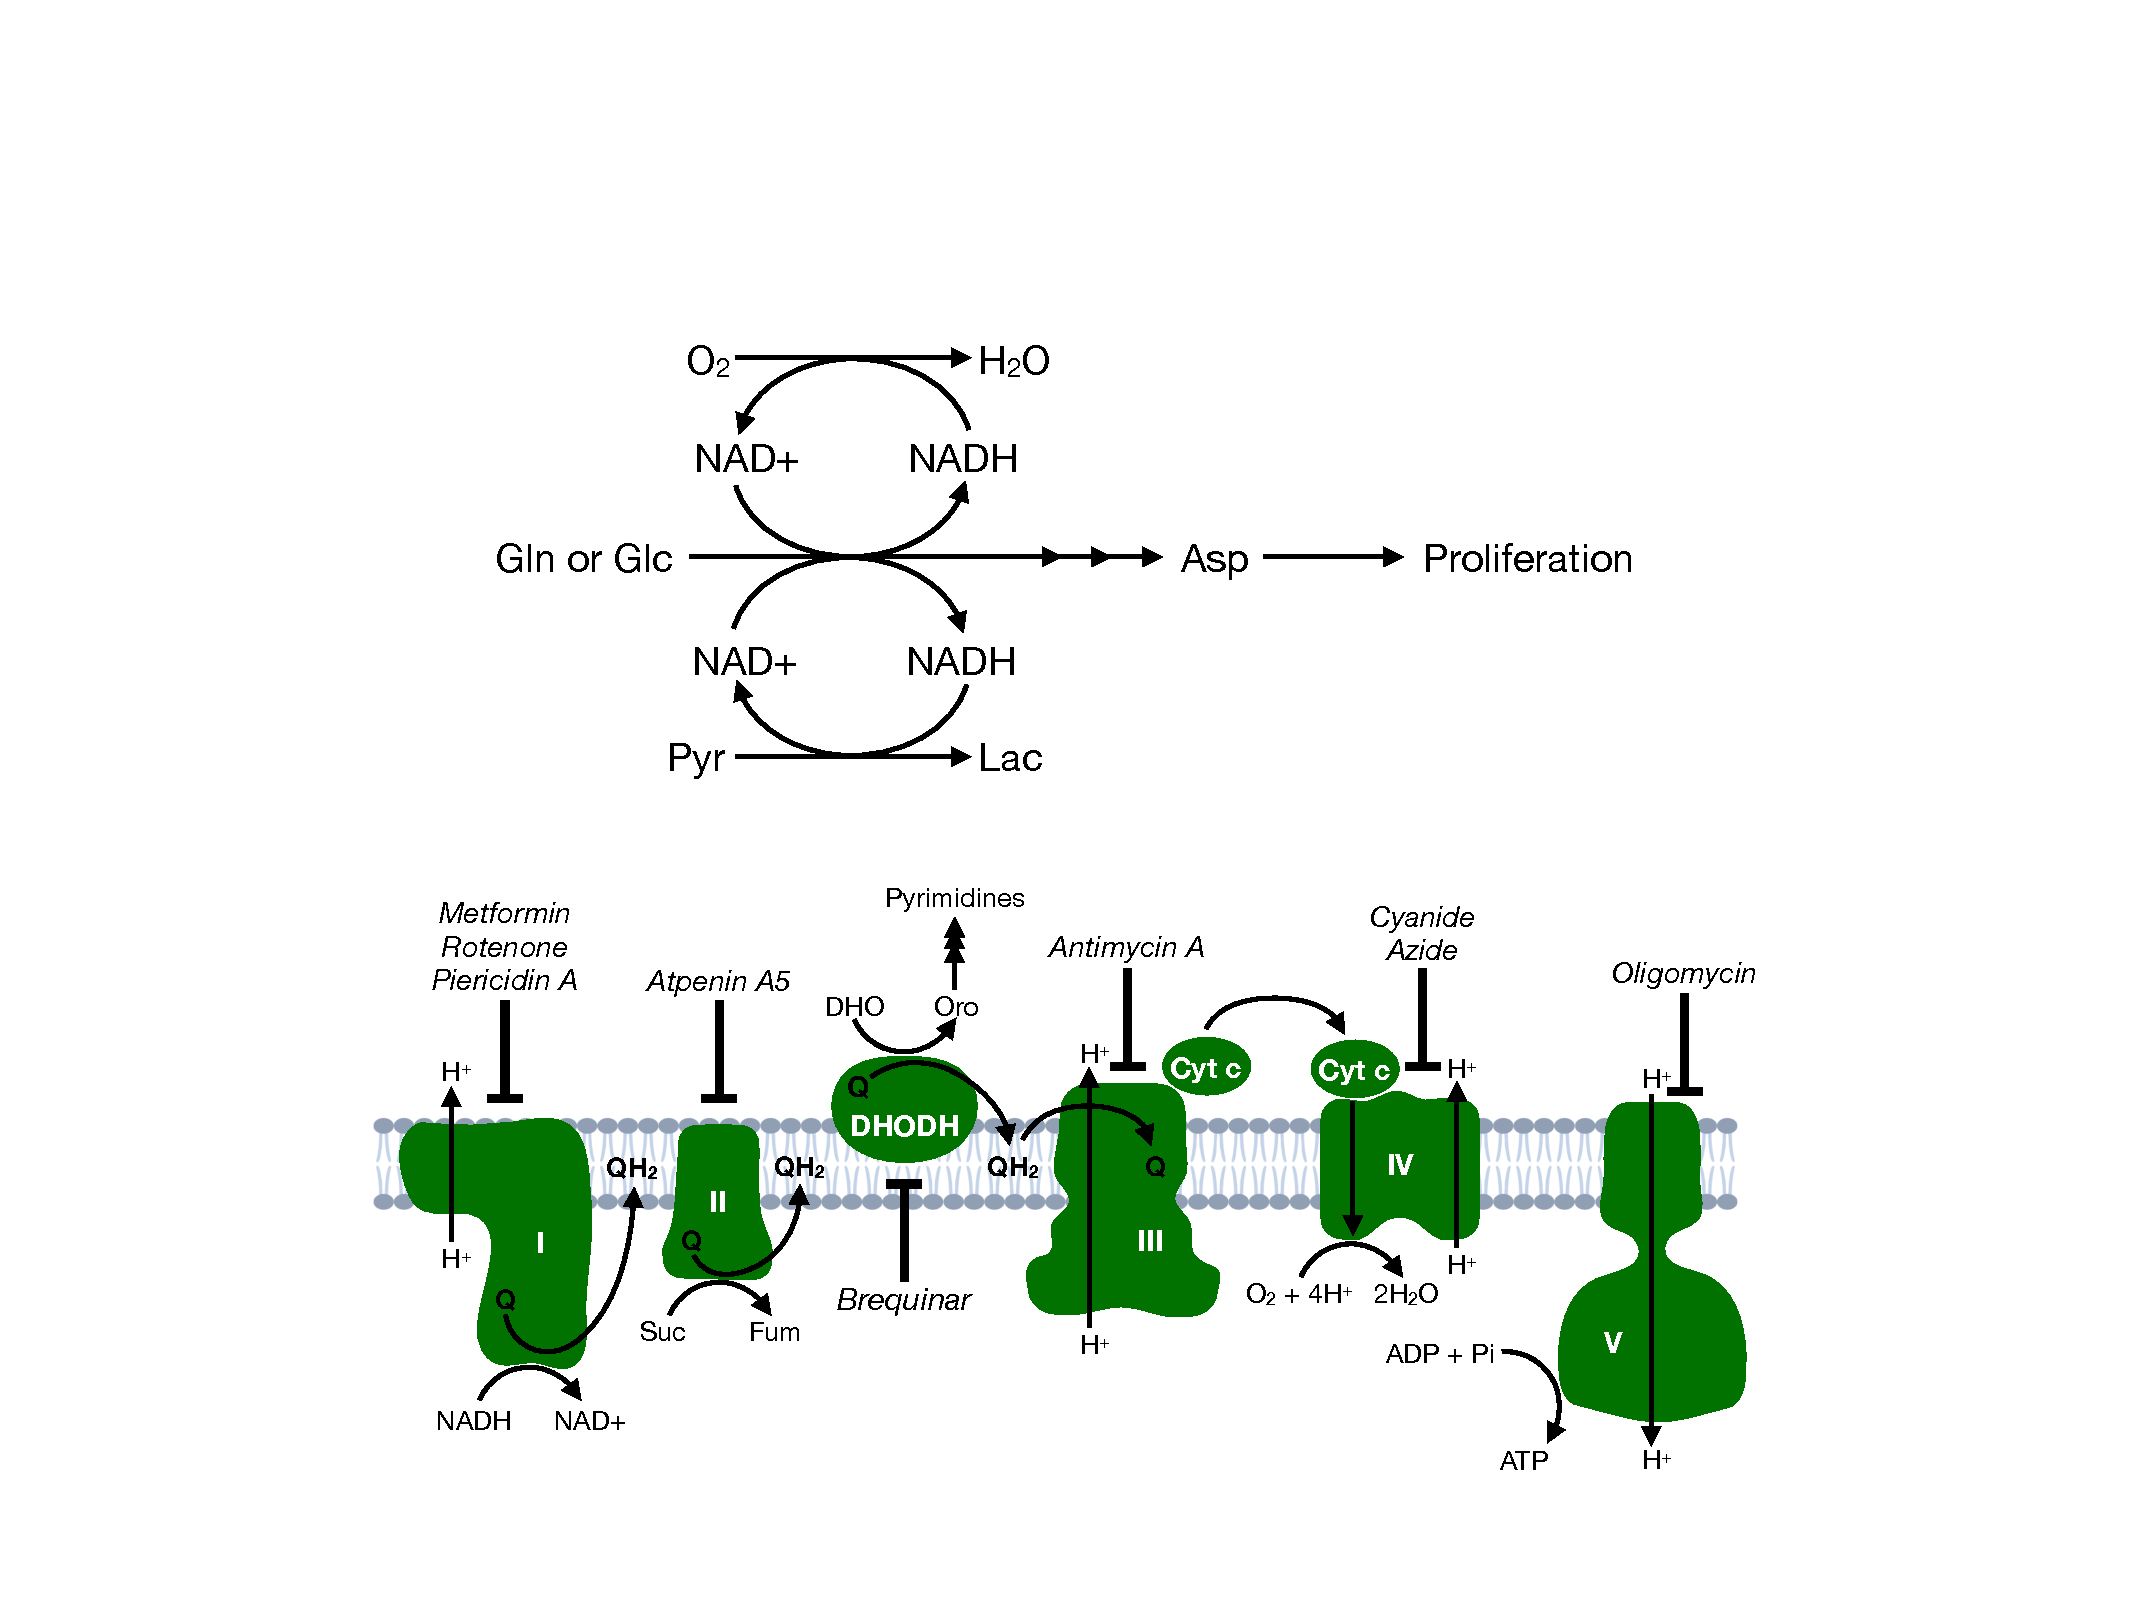
\includegraphics[width=0.70\textwidth]{figures/chap1/redox_biomass.pdf}
    \caption[Biomass accumulation requires \NAD{} regeneration.]{
    Biomass accumulation requires \NAD{} regeneration.
    Top diagram: glutamine or glucose is converted into aspartate with consumption of \NAD.
    Aspartate synthesis is necessary for cell proliferation as it cannot be scavenged from the environment, therefore \NAD{} regeneration is required either through respiration using oxygen or with an electron acceptor such as pyruvate.
    Bottom diagram: the mitochondrial electron transport chain regenerates \NAD{} through respiration of oxygen and many inhibitors exists to probe the effect of each component in the chain.
    }
    \label{fig:ch1:redox_biomass}
\end{figure}


Aspartate synthesis appears to be at the nexus of redox imbalance due to its inability to be scavenged from the environment and thus the aspartate level, the \NAD/NADH ratio and cell proliferation is coupled together.
This coupling has been observed when progressively inhibiting respiration such that the \NAD/NADH ratio decreases from baseline.
A sigmoidal relationship between \NAD/NADH ratio and proliferation is observed; however, the \NAD/NADH ratio is also tightly correlated with intracellular aspartate levels \cite{Gui2016-ca}.
This raises the question of causality: is proliferation decrease cause by aspartate or the \NAD/NADH ratio?

The evidence is now clear that aspartate is the cause of limited proliferation.
Large parts of the proliferation defects caused by inhibiting respiration can be rescued by directly supplying the cells with aspartate either through supraphysiological concentrations (20-40 mM) \cite{Gui2016-ca, Birsoy2015-pg, Sullivan2015-xf, Krall2021-mb} or expression of an aspartate transporter or an asparaginase enzyme \cite{Birsoy2015-pg, Pavlova2018-nl, Garcia-Bermudez2018-mj, Sullivan2018-gz}.
Respiratory deficient cells, either depleted of mitochondrial DNA ($\rho^0$) or having a frameshift deletion in cytochrome B (CytB), have also been rescued using aspartate \cite{Sullivan2015-xf, Birsoy2015-pg}.
Aspartate limitation can also be induced through complex II inhibition which prevents succinate oxidation to fumarate and thus stops TCA cycling and mitochondrial aspartate synthesis.
In this case, when cells are provided with an electron acceptor like pyruvate, the cytoplasmic \NAD/NADH ratio is rescued but proliferation is not, and it is only by increasing the intracellular aspartate concentration that proliferation is rescued \cite{Hart2023-gp}, thus uncoupling the \NAD/NADH ratio from proliferation.

In figure \ref{fig:ch1:redox-prlfr_uncpl} such uncoupling experiment is repeated by expression of the Glu/Asp transporter SLC1A3 after which aspartate can be delivered by media addition.
Using complex I inhibitor rotenone to suppress respiration and thus decreasing proliferation and the \NAD/NADH ratio, proliferation was almost fully rescued by aspartate delivery, thus confirming that proliferation is limited by aspartate and not \NAD.

\begin{figure}
    \centering
    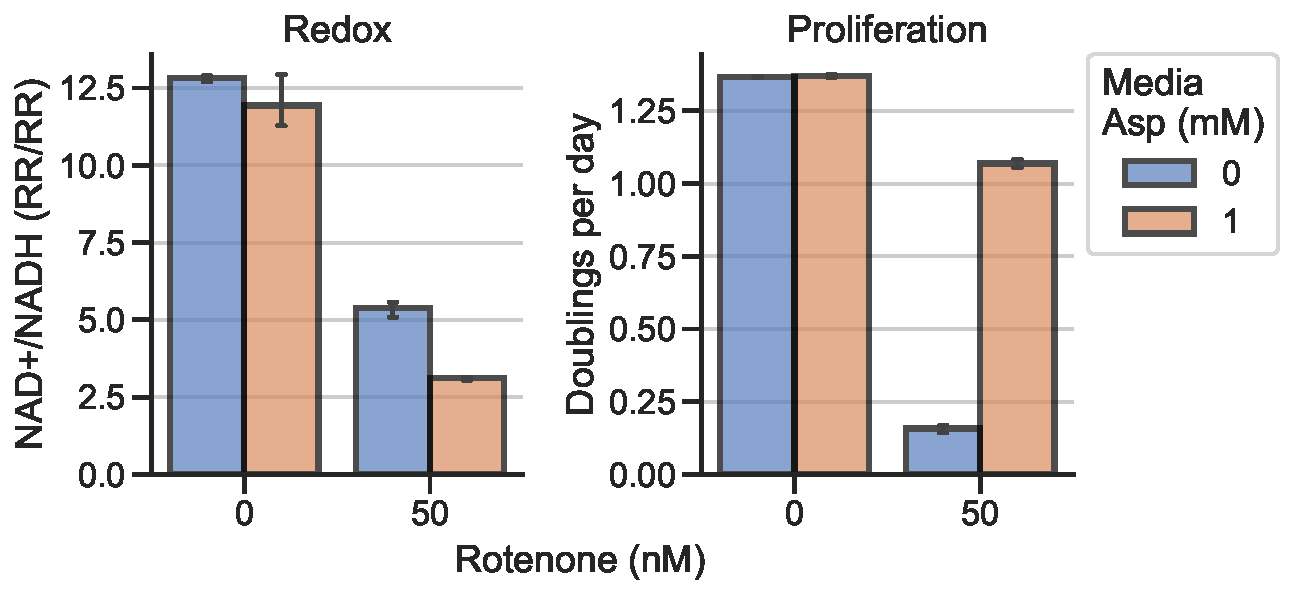
\includegraphics[width=0.70\textwidth]{figures/chap1/redox-prlfr_uncpl.pdf}
    \caption[Aspartate rescues proliferation but not the \NAD/NADH ratio.]{
    Aspartate rescues proliferation but not the \NAD/NADH ratio.
    Uncoupling \NAD/NADH and aspartate's effect on proliferation using 143B cells with stable expression of the Glu/Asp transporter SLC1A3, treated with/without 1 mM media aspartate and with/without 50 nM rotenone.
    \NAD/NADH ratio measured using LCMS as a ratio between two internal standard normalized response ratios (RR/RR).
    }
    \label{fig:ch1:redox-prlfr_uncpl}
\end{figure}


In summary, aspartate synthesis is required for cell proliferation due to its impermeability, its synthesis consumes \NAD{} thereby coupling it to respiration, it appears to be insufficiently synthesized by tumors limiting their growth and it is limiting cell proliferation during respiration deficiency.
This has prompted us to investigate which fate of aspartate is responsible for limiting tumor growth and cell proliferation.



\section{Aspartate fates}
Amino acids can be divided into two groups: terminal amino acids such as asparagine, threonine, valine, leucine, histidine, tryptophan etc. which only fate is protein synthesis and metabolized amino acids such as serine and methionine in the folate and methionine cycles, glutamate as a substrate for anaplerosis and glutamine as a nitrogen donor.
However, notice that this grouping will change depending on the cell context e.g. in certain cells and conditions valine, leucine and isoleucine will be consumed as a substrate for anaplerosis, tryptophan will fuel the kynurenine pathway etc.
Therefore, when discussing the fates of an amino acid, or any metabolite, the cell context must be considered to focus attention on relevant pathways and avoid getting lost in the vast metabolic network.

For aspartate the relevant fates are asparagine and nucleotide synthesis (figure \ref{fig:ch1:asp_fates}).
For nucleotide synthesis, aspartate is consumed to make pyrimidine precursor carbamoyl-aspartate, in the purine synthesis pathway to make purine precursor IMP and in the conversion of IMP to AMP.
Aspartate fates can be divided into two classes: fates consuming the aspartate carbon backbone and fates where only the nitrogen is donated, and the carbon backbone is returned in the form of fumarate.
The distinction is important as fumarate has the same redox state as aspartate and can be recycled back into aspartate with no net consumption of \NAD (appendix \ref{fig:app_ch1:fumarate_NAD}).
On the other hand when aspartate is consumed for asparagine, pyrimidine or protein synthesis it must be replenished by synthesis from glucose or glutamine at the cost of \NAD{} consumption.

Aspartate is a nitrogen donor in the urea cycle, required to convert citrulline into arginine.
For cells synthesizing their own arginine, this is drained from the urea cycle which is then replenished by ornithine synthesis from glutamate and subsequent conversion to citrulline by ornithine transcarbamylase to close the cycle.
However, ornithine transcarbamylase is almost exclusively expressed in the liver and gastrointestinal tract, with no expression in most cancer cell lines; therefore, non-hepatic cell lines have no net arginine synthesis and are arginine auxotrophs unless provided with exogenous citrulline.

N-acetylaspartate is another potential aspartate fate found abundantly in brain tissue but also to some extend in adipocytes; however, most other tissues and cancer cell lines do not produce appreciable amounts of N-acetylaspartate.
This correlates with lacking expression of NAT8L, the enzyme responsible for its synthesis \cite{Alkan2020-td}.
Therefore, in the context of cancer cell lines, N-acetylaspartate does not consume a meaningful amount of aspartate, nor is it a metabolite that appear to influence cell proliferation.

Finally, although not a net consumption term, aspartate is used as a shuttle metabolite in the aspartate-malate shuttle to transfer electrons generated in the cytoplasm into the mitochondrial matrix.

\begin{figure}
    \centering
    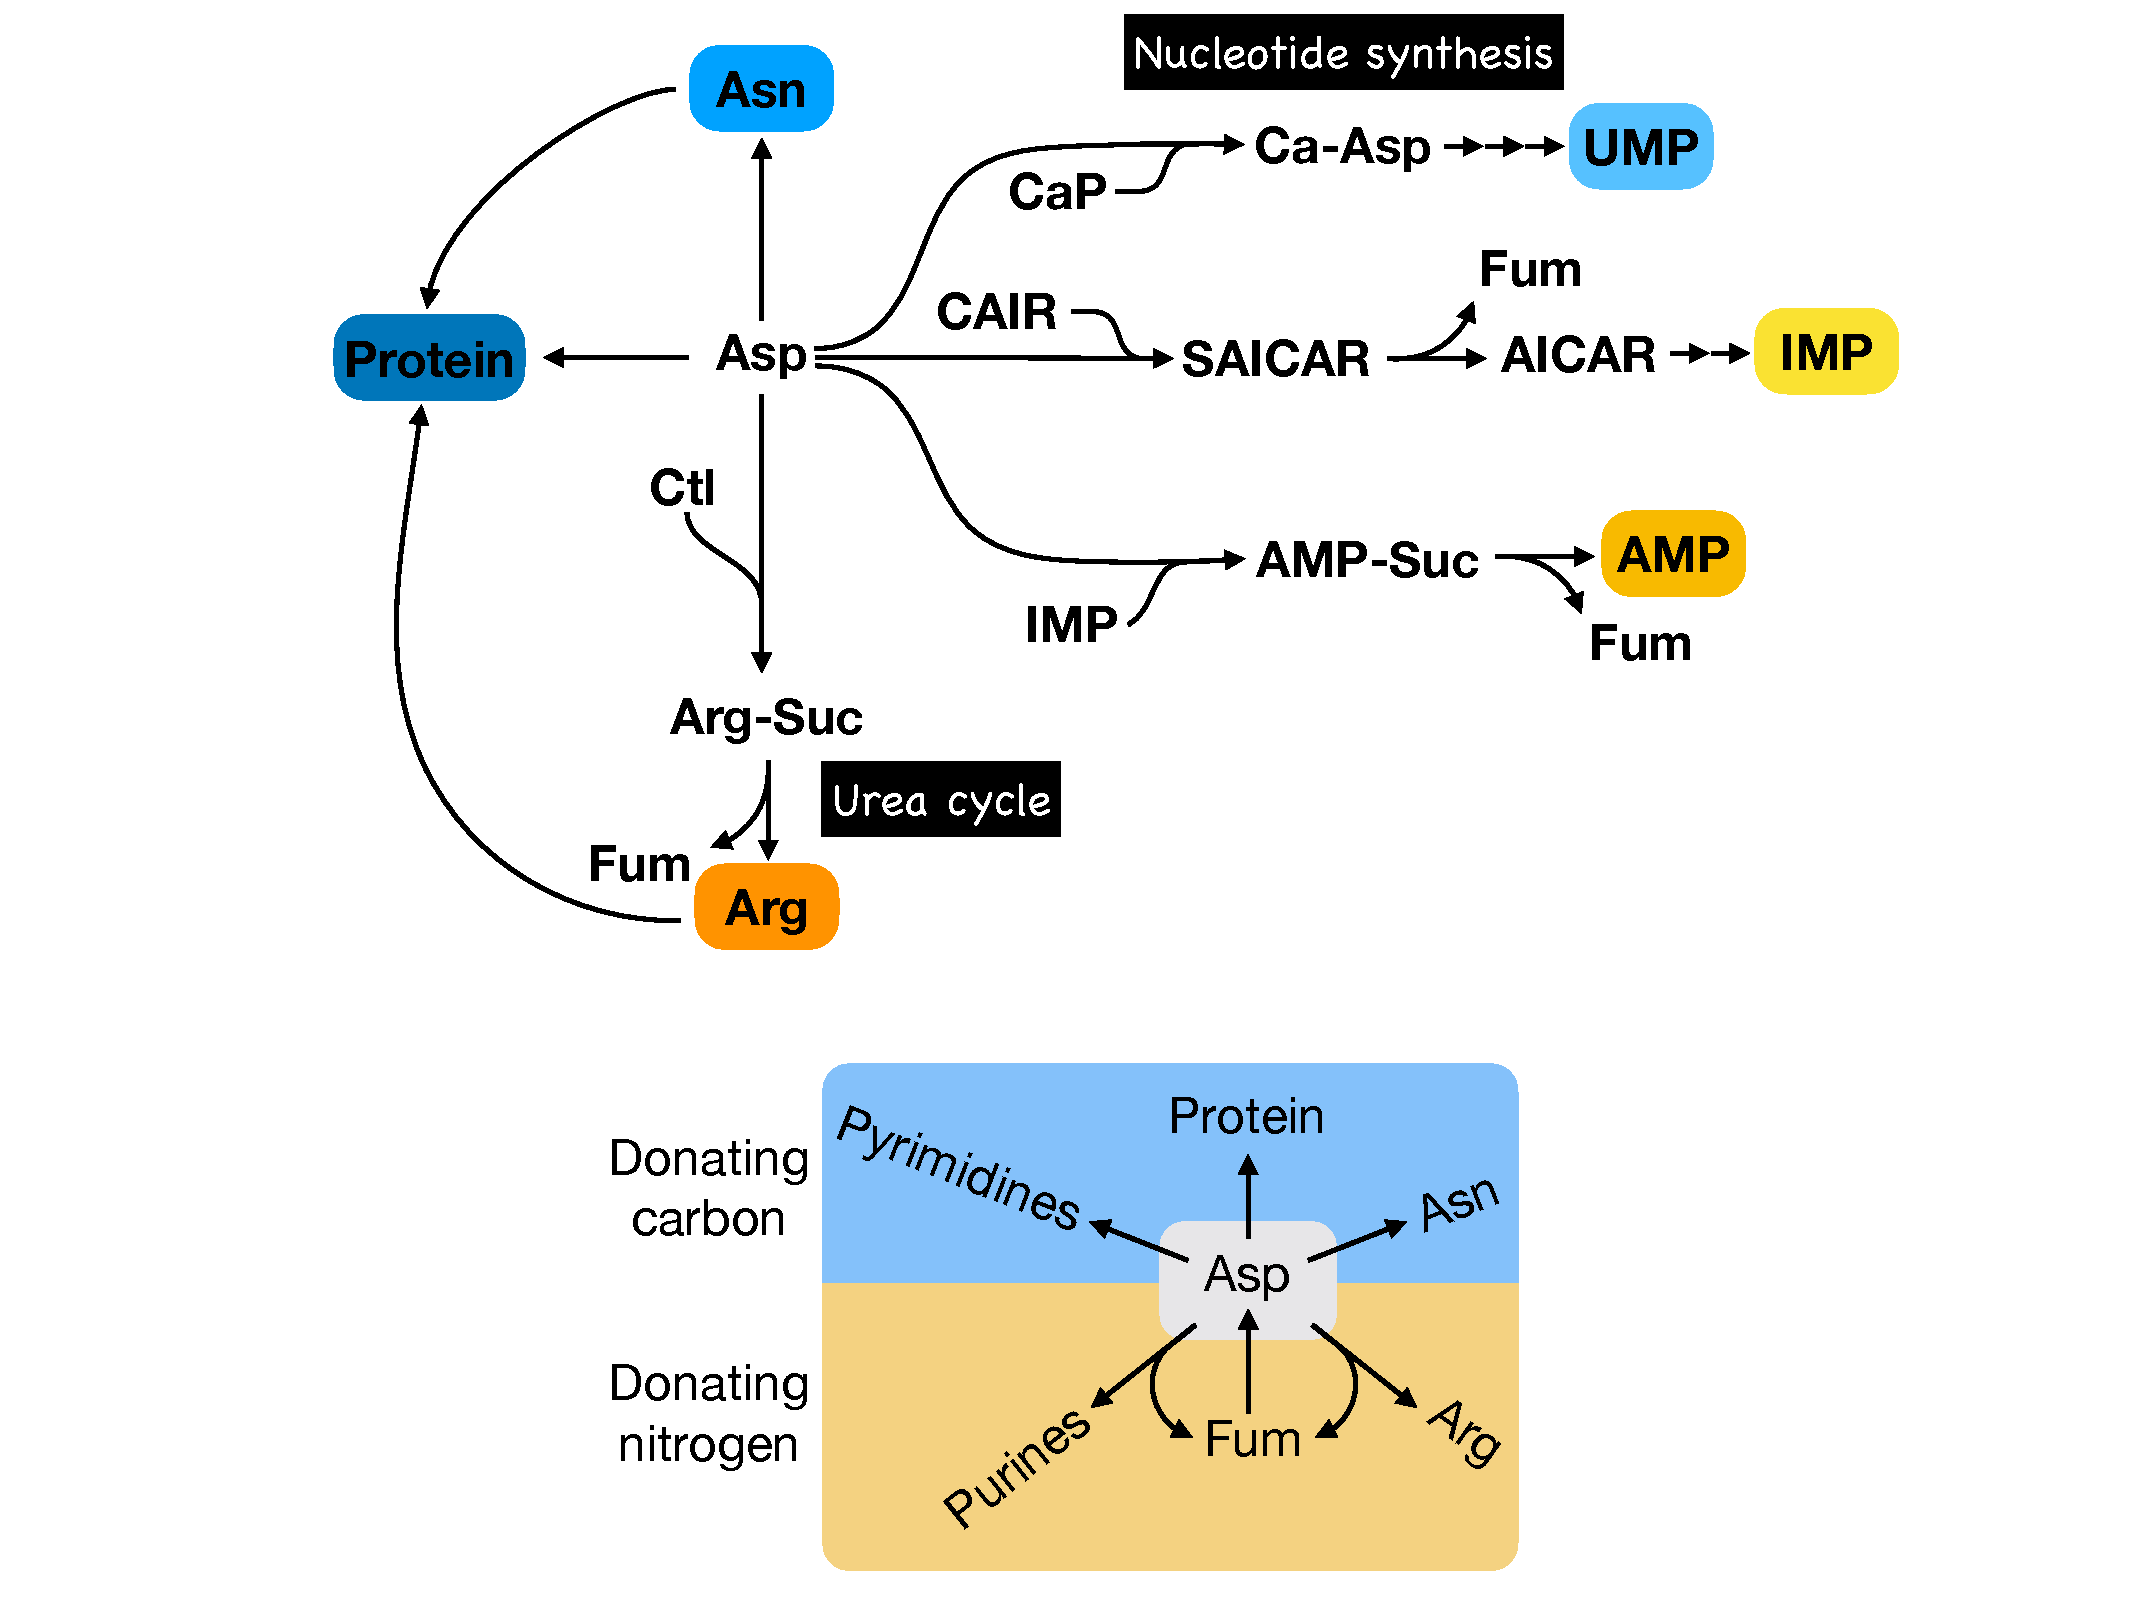
\includegraphics[width=0.70\textwidth]{figures/chap1/asp_fates.pdf}
    \caption[Metabolic fates of aspartate.]{
    Metabolic fates of aspartate.
    Top diagram: aspartate is used as a substrate for protein synthesis directly and indirectly as a precursor of asparagine and arginine.
    Aspartate is also a substrate for all pyrimidine synthesis, synthesis of purine precursor IMP and conversion of IMP to AMP.
    Bottom diagram: aspartate fates can be divided into those where aspartate is donating its carbon backbone and thus requiring \NAD{} consumption to resynthesize aspartate (pyrimidine, protein and asparagine synthesis) and those where aspartate is donating its amino group nitrogen to yield fumarate which can be recycled back to aspartate in a redox neutral way.
    }
    \label{fig:ch1:asp_fates}
\end{figure}




\subsection{Aspartate metabolism fluxes}
Each aspartate fate is responsible for a fraction of the total cellular aspartate consumption, a consumption rate also known as a flux.
These aspartate consumption fluxes could change in different conditions such as during mitochondrial inhibition or when aspartate fates can be salvaged from the environment and thus measuring each flux would be useful tool.
Flux measurements are often done using stable isotope tracing and are routinely applied using \hCi{}-labelled glucose, glutamine or other amino acids \cite{Yuan2008-eu, Park2016-ap, Jang2018-ey, Bartman2021-ey}.

As such, flux can easily be calculated by measuring label incorporation over time e.g. if labelled metabolite $A$ is introduced at time zero and consumed to synthesize labelled metabolite $B$ then the label incorporation is described by an exponential with the rate $r_{AB}$ and pool size $[B]$:
$$
B_{\text{labelled}}(t) = [B] - [B] e^{-r_{AB} t}
$$
The synthesis flux is defined as: $F_{syn} = [B] r_{AB}$ and controls the time before half of the pool is labelled:
$$
t_{1/2} = \frac{[B]}{F_{syn}} \ln(2)
$$
A detailed treatment of this example can be found in appendix \ref{chap1_app:flux}.

In these simple flux measurements, it is assumed that the reaction is irreversible, but it is trivial to extend the mathematical model to a reversible reaction; however, it is not always trivial to measure the flux of such reversible reactions.
Unfortunately, this is the case for the fates of aspartate which has several challenges.
Firstly, the impermeability makes it impractical to use aspartate directly as a tracer, and secondly, aspartate fates both involve carbon and nitrogen.
Potentially, both of these issues could be solved using U-\hCi{}, U-\hNi{} glutamine but the number of relevant reaction rates is very large (figure \ref{fig:ch1:asp_fluxes}) and to solve such system it would be necessary to measure protein, DNA and RNA abundance and breakdown rates.
This makes aspartate fate flux very difficult to measure directly using time-series of isotopic labelling and therefore were not attempted.
Instead, fluxes were estimated using measurements of total amino acids and nucleotides at a steady-state proliferation rate (detailed in chapter \ref{chap2}).

\begin{figure}
    \centering
    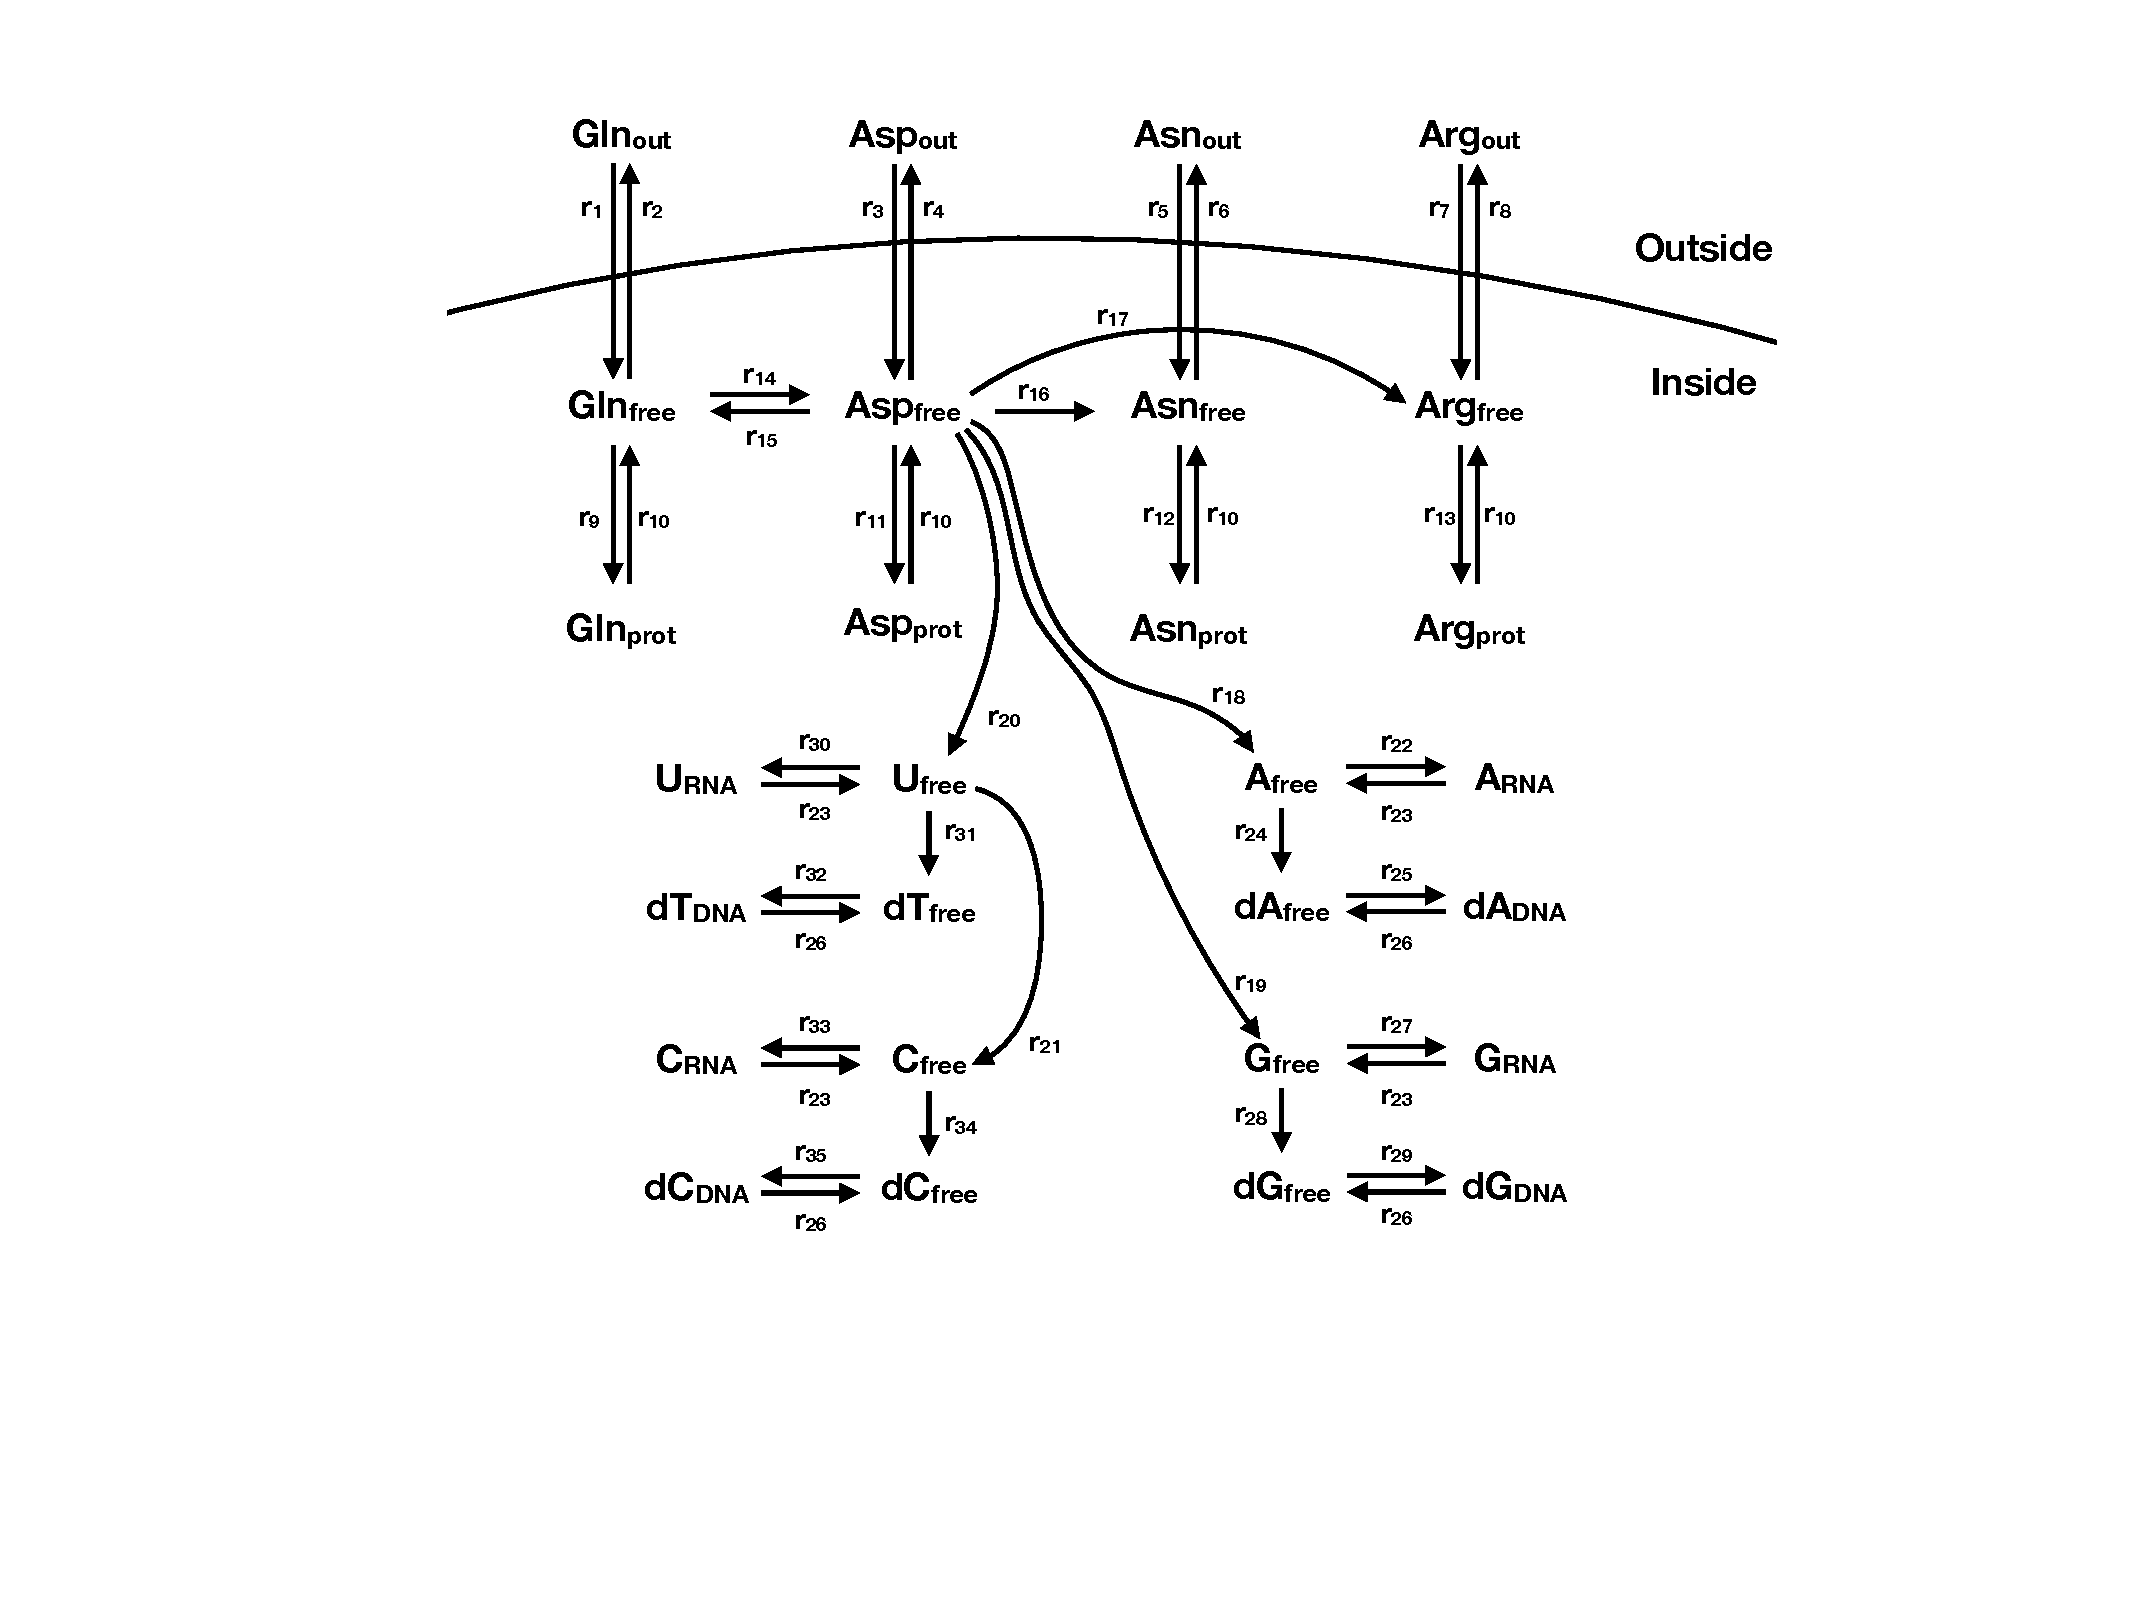
\includegraphics[width=0.70\textwidth]{figures/chap1/asp_fluxes.pdf}
    \caption[Aspartate metabolism fluxes.]{
    Aspartate metabolism fluxes as they would appear from glutamine labelling with enumerated conversion rates.
    Amino acids are either outside the cell (out), inside the cell (free) or bound in protein (prot).
    Nucleotides are either as (d)NTP, (d)NDP, (d)NMP free or bound in RNA/DNA.
    }
    \label{fig:ch1:asp_fluxes}
\end{figure}





\section{Which aspartate fate controls proliferation}
Based on the fates of aspartate it can be speculated which of these, if any, is ``the first-degree effect'' responsible for the relationship between aspartate and proliferation.
As tumor growth is aspartate limited is seems likely that tumors are also experiencing this first-degree effect of aspartate limitation, whatever it may be.
Several of the metabolic fates of aspartate can be salvaged from the environment e.g. asparagine, uridine, hypoxanthine and adenine to complement asparagine, pyrimidine IMP and AMP synthesis, respectively.
And thus, if depletion of any one of the salvageable aspartate fates is the first-degree effect of aspartate limitation, then it can be added to the media to either rescue proliferation or induce a further aspartate depletion resulting in a ``second degree effect'' which then controls proliferation.
In both cases the aspartate to proliferation rate correlation would be shifted to reflect that proliferation is no longer mediated by the first-degree effect.

Initially, the effect of all salvageable fates of aspartate can be tested with a ``Salvage mix'' containing these at a sufficient concentration.
This tests the hypothesis that one of the aspartate fates is the first-degree effect of aspartate limitation.
Thus, if this fate is scavenged through salvage mix supplementation it enables proliferation at lower a aspartate concentration (figure \ref{fig:ch1:asp_fates_suppl_hypo}).
If true, this fate can by isolated by attempting proliferation rescue with single components from the salvage mix.
If false, none of the salvageable fates is the first-degree effect of aspartate limitation, leaving aspartate consumption to protein.

\begin{figure}
    \centering
    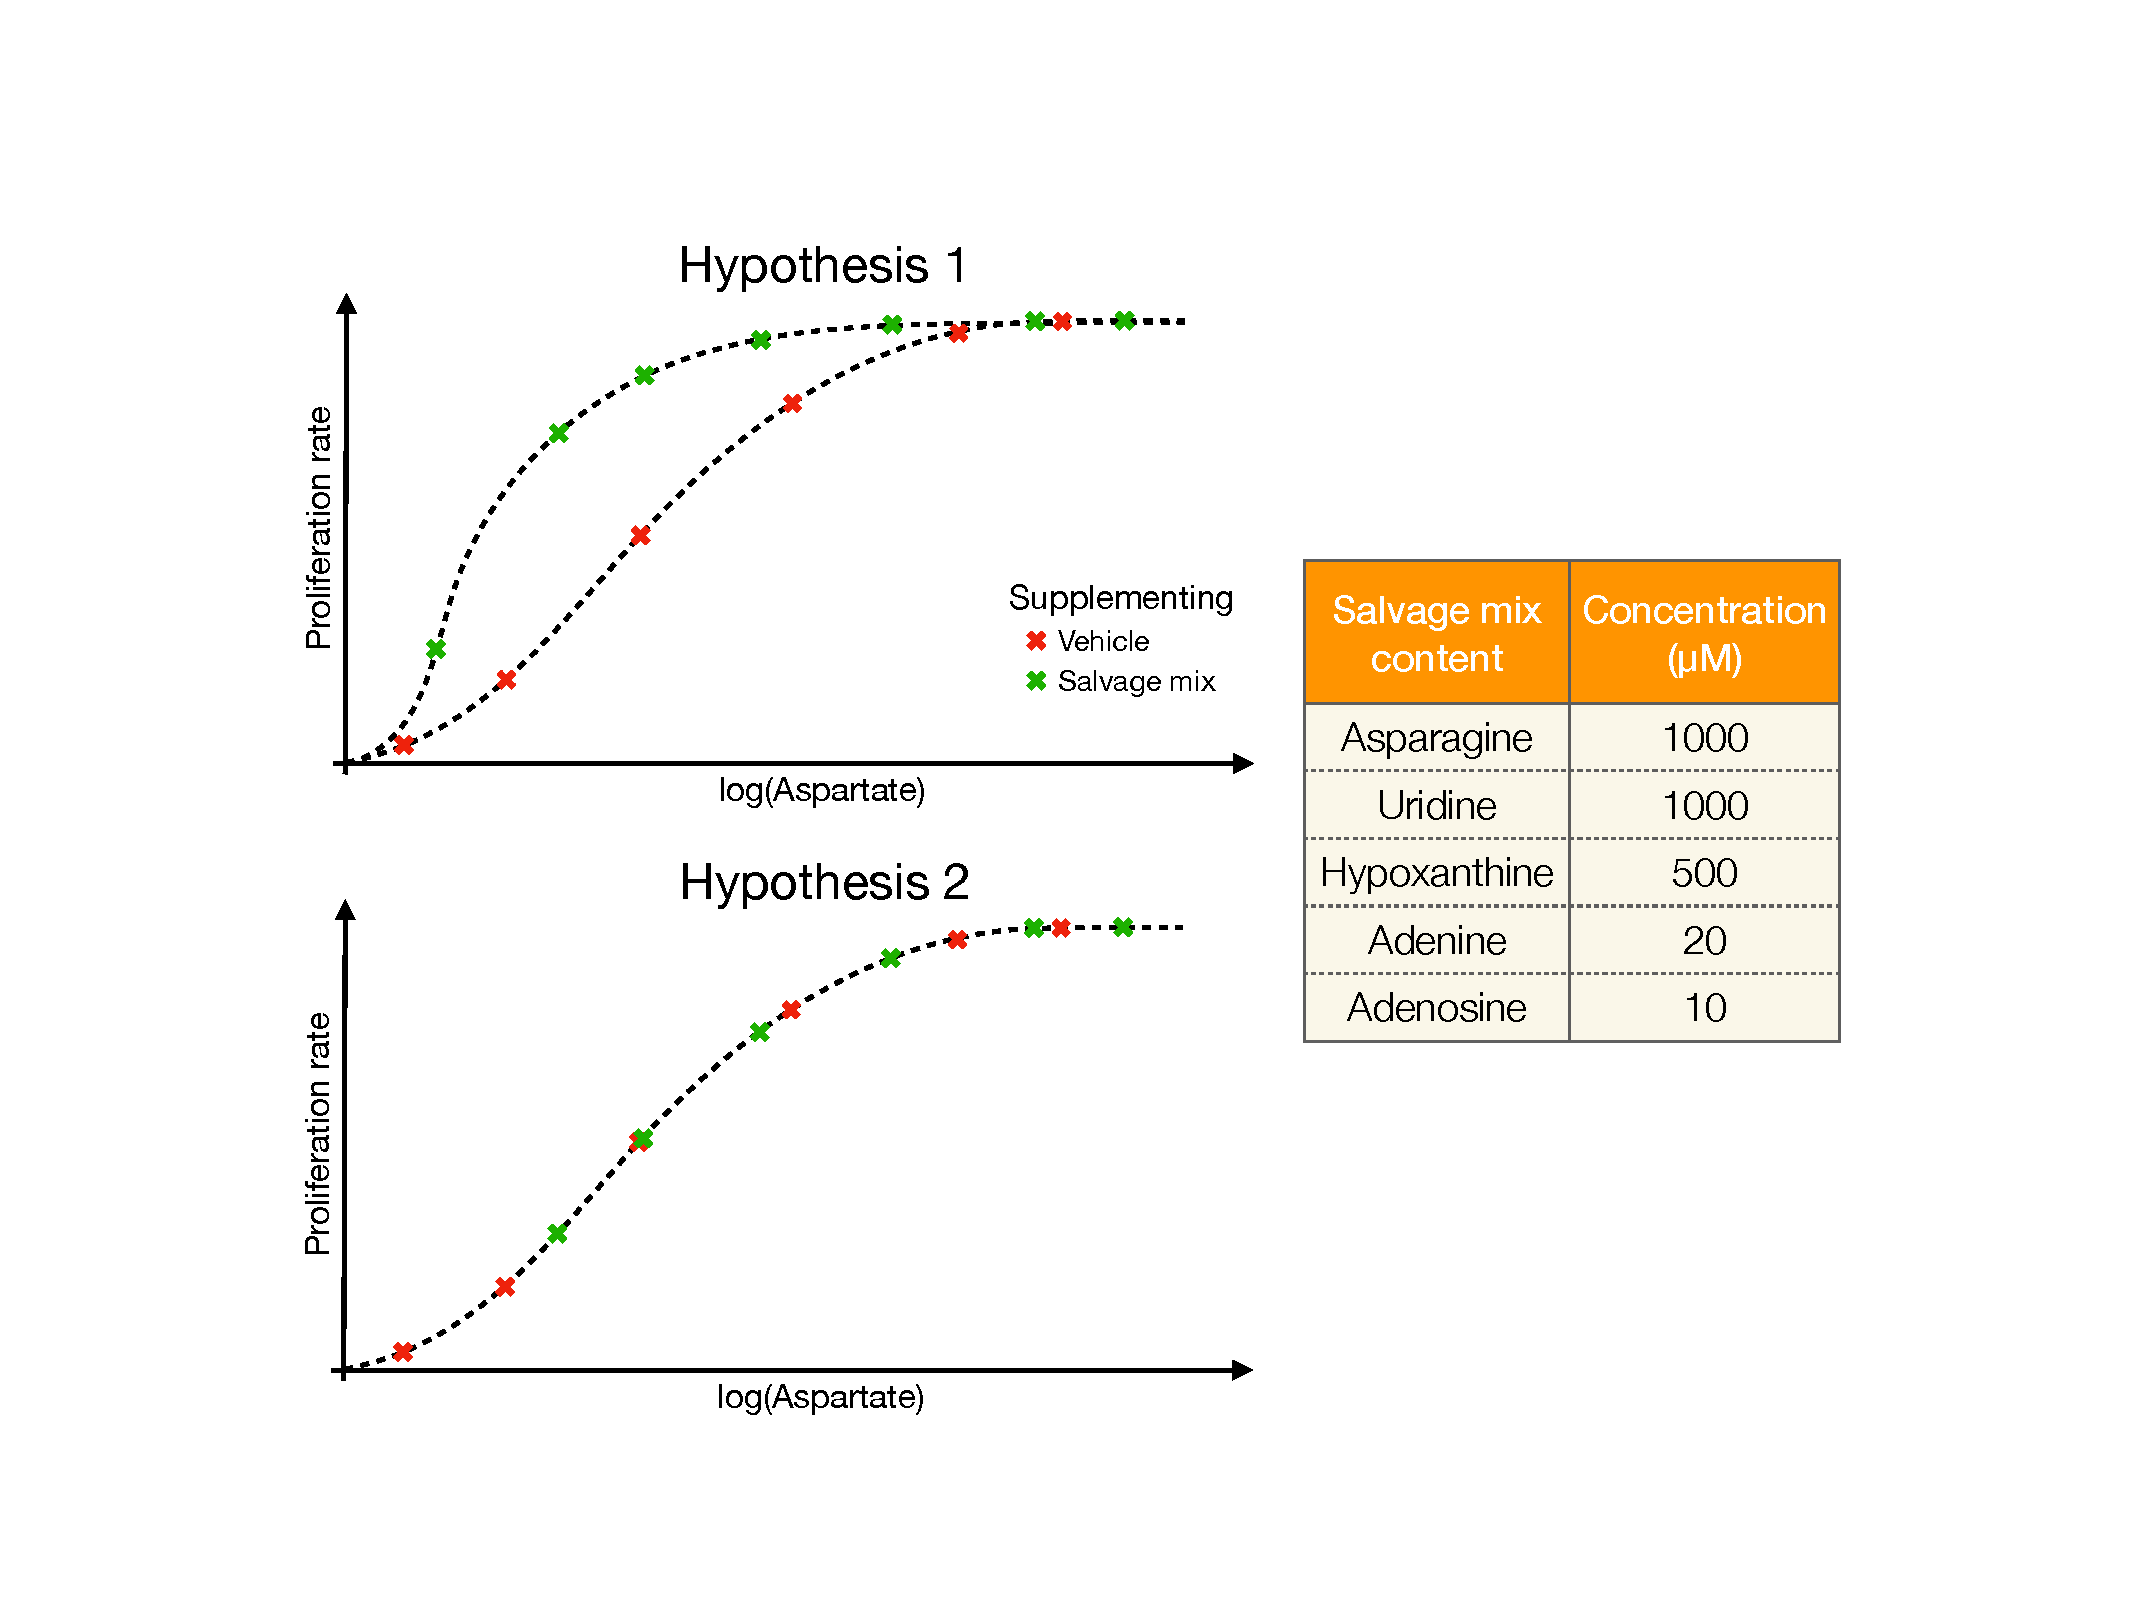
\includegraphics[width=0.70\textwidth]{figures/chap1/asp_fates_suppl_hypo.pdf}
    \caption[Two hypotheses for aspartate to proliferation correlation.]{
    Two hypotheses for aspartate to proliferation correlation.
    Hypothesis 1 posits that some fate of aspartate is the direct cause of aspartate limited proliferation and thus if this fate is scavenged through salvage mix supplementation it enables proliferation at a lower aspartate concentration.
    Hypothesis 2 posits that no such fate exists, or that it cannot be scavenged through salvage mix supplementation.
    }
    \label{fig:ch1:asp_fates_suppl_hypo}
\end{figure}







